 \chapter{Разработка алгоритмов геолокации с помощью глубокого обучения}

В этой главе описываются разработанные/модифицированные модели/методы/
алгоритмы, или/и описывается применение известных стандартных методов. Также, 
в конце главы обычно приводится общая архитектура программной системы, 
вытекающая из описанной теории. Приведенные ниже заголовки подразделов так же 
весьма примерные и сильно зависят от особенностей конкретной работы.
\section{Формальная постановка задачи геолокации по серии изображений}

Задача геолокации (визуальной локализации) в данном исследовании ставится как задача классификации изображений местности в соответствующие им области земной поверхности. Более формально, пусть:

\begin{compactitem}
	\item $K$ --- число ячеек в которых могли быть сделаны фотографии,
	\item $N$ --- число фотографий,
	\item $m_i$ --- число фотографий в $i$-том альбоме,
	\item $ Q $ --- число альбомов,
	\item $X$ --- множество фотографий. 
	\item $ Y $ --- множество ячеек, 
	\item $ s2(\gamma) $ --- сопоставление GPS координатам $ \gamma $ ячейке из $ Y $. Для обучающей выборки известны значения $ s2^{-1} $, то есть отображения $ y \to \gamma $
\end{compactitem}
ячейка --- область земной поверхности, выделенная например с помощью S2 разбиения,\\
фотография --- тензор\, $ l \times q \times 3$  действительных чисел, $ l, q $ --- ширина 
и высота соответственно\footnote{индексы фотографии для простоты опущены},\\
альбом --- упорядоченный набор из $ m_i $ фотографий объединённых по признаку нахождения в одной ячейке, 
$ K, N, Q $ определяются обучающей выборкой.

Обучающая выборка --- множество пар <<фотография --- ячейка>>, $\mathbf{X} = \left\{(X_j, y_j)|j = 1 .. N \right\} $, возможно объединённые в альбомы по $ m_j $ штук.

Требуется разработать:
\begin{compactitem}

\item алгоритм, $ \mathcal{F}: X \to Y $
который будет сопоставлять элементу $ x_j $ класс $ \hat{y}_j $ наиболее близкий к тому которым $ x_j $ обладает в реальности, c набором параметров $ W_1 $
\item алгоритм $ \mathcal{G}: [X] \to Y $, где $ [x] $ --- список $ x $, решающий эту задачу для альбома,  $ \mathcal{G}$ обладает набором параметров $ W_2 $

\end{compactitem}

Обучение $ \mathcal{F} $ и $ \mathcal{G} $ состоит в подборе наборов параметров $ W_1 $ и $ W_2 $. Следует отметить что целесообразно использовать для реализации $ \mathcal{G} $ параметры $ \mathcal{F} $, а значит $ W_2 $ --- суть $ W_1 $ и параметры, специфичные для обработки последовательностей. Оптимальные значения параметров $ W_1 $ и $ W_2$ зависят от обучающей выборки.

Таким образом можно рассматривать $ \mathcal{F} $ и $ \mathcal{G} $
как отображение обучающей выборки в множество функций, отображающих в $ Y $ .

Следует также отметить что частота разбиения поверхности может быть различной, а значит для каждого масштаба возможно обучать различные версии $ \mathcal{F}  $ и $ \mathcal{G} $.

Для простоты будем считать что перед подачей на вход алгоритмам изображения масштабируются и обрезаются если требуется. Процесс масштабирования будет описан ниже.

\section{Выбор/разработка методов оценки точности работы алгоритмов геолокации}

Для получения нижней оценки на точность алгоритма можно рассматривать в качестве ошибки предсказания расстояние от центра ячейки $ С(\hat{y}) $ до реальных GPS координат фотографии $ s2^{-1}(y) $, рассчитанное по поверхности земли $ d(a,b) $.

Тогда ошибкой для выборки будет
$$ E = \frac{1}{K} \sum_{i=1}^{K} {d(y_{j},C(\hat{y_j}))}$$

Для обучения будем использовать скользящий контроль.

%TODO go on . . .

\section{Модификация существующих решений в области для работы с серией изображений}

Хотя разрабатываемая архитектура способна локализовать большое разнообразие изображений, многие изображения неоднозначны или не предоставляют достаточно информации, которая позволила бы их локализовать.
Однако мы можем использовать тот факт, что фотографии естественным образом происходят в последовательности, например, альбомы, место съёмки которых часто значительно скоррелировано. Интуитивно, если мы с уверенностью можем локализовать
некоторые из фотографий в альбоме, мы можем использовать эту информацию,
чтобы локализовать фотографии с неопределенным местоположением. Фотографии в альбоме --- это последовательность,
которая требует модели, которая запоминает состояние предыдущего примера, 
при рассмотрении текущего примера. Поэтому целесообразно использовать
(LSTM) \cite{hochreiter1997long} для этой задачи.
Теперь мы рассмотрим, как решить проблему прогнозирования
геолокации последовательности фотографий с использованием LSTM.


\subsection{Сети LSTM}

Долгая краткосрочная память (Long short-term memory; LSTM) – особая разновидность архитектуры рекуррентных нейронных сетей, способная к обучению долговременным зависимостям. Они были представлены Зеппом Хохрайтер и Юргеном Шмидхубером (Jürgen Schmidhuber)\cite{hochreiter1997long} в 1997 году, а затем усовершенствованы и популярно изложены в работах многих других исследователей. Они прекрасно решают целый ряд разнообразных задач и в настоящее время широко используются.

LSTM разработаны специально, чтобы избежать проблемы долговременной зависимости. Поэтому запоминание информации на долгие периоды времени легко реализуется данной архитектурой.

Опишем основную операцию генератора паттренов на основе LSTM\cite{gers1999learning}:
Блок LSTM имеет механизмы, позволяющие «запоминать» информацию для расширенного количества временных шагов. Мы используем блок LSTM со следующими преобразованиями, которые отображают входы для выходов по блокам в последовательных слоях и последовательных временных шагах:

\[
{\displaystyle {\begin{aligned}
	f_{t} & =\sigma _{g}(W_{f}x_{t}+U_{f}h_{t-1}+b_{f})                               \\
	i_{t} & =\sigma _{g}(W_{i}x_{t}+U_{i}h_{t-1}+b_{i})                               \\
	o_{t} & =\sigma _{g}(W_{o}x_{t}+U_{o}h_{t-1}+b_{o})                               \\
	c_{t} & =f_{t}\circ c_{t-1}+i_{t}\circ \sigma _{c}(W_{c}x_{t}+U_{c}h_{t-1}+b_{c}) \\
	h_{t} & =o_{t}\circ \sigma _{h}(c_{t})
\end{aligned}}}
\]

где $ \circ $ - оператор поэлементного умножения, и две функции активации:
\[\begin{aligned}
 \sigma(\mathbf{x_i}) & =\frac{1}{1+e^{-\mathbf{x_i}}} \, \\
 \tanh(\mathbf{x_i}) & =\frac{1-e^{-2\mathbf{x_i}}}{1+e^{-2\mathbf{x_i}}} \\
 \end{aligned}
\]

Переменные:
\begin{itemize}
\item $ {\displaystyle x_{t}} $ — входной вектор,
\item $ {\displaystyle h_{t}}  $ — выходной вектор,
\item $ {\displaystyle c_{t}}  $ — вектор состояний,
\item $ {\displaystyle W } $ , $ {\displaystyle U }$ и $ {\displaystyle b} $ — матрицы параметров и вектор,
\item $ {\displaystyle f_{t}}  $, $ {\displaystyle i_{t}} $ и $ {\displaystyle o_{t}} $ — векторы вентилей,
\item $ {\displaystyle f_{t}}  $ — вектор вентиля забывания, вес запоминания старой информации,
\item $ {\displaystyle i_{t}}  $ — вектор входного вентиля, вес получения новой информации,
\item $ {\displaystyle o_{t}} $ — вектор выходного вентиля, кандидат на выход.
\end{itemize}
\begin{figure}[h]
	\centering
	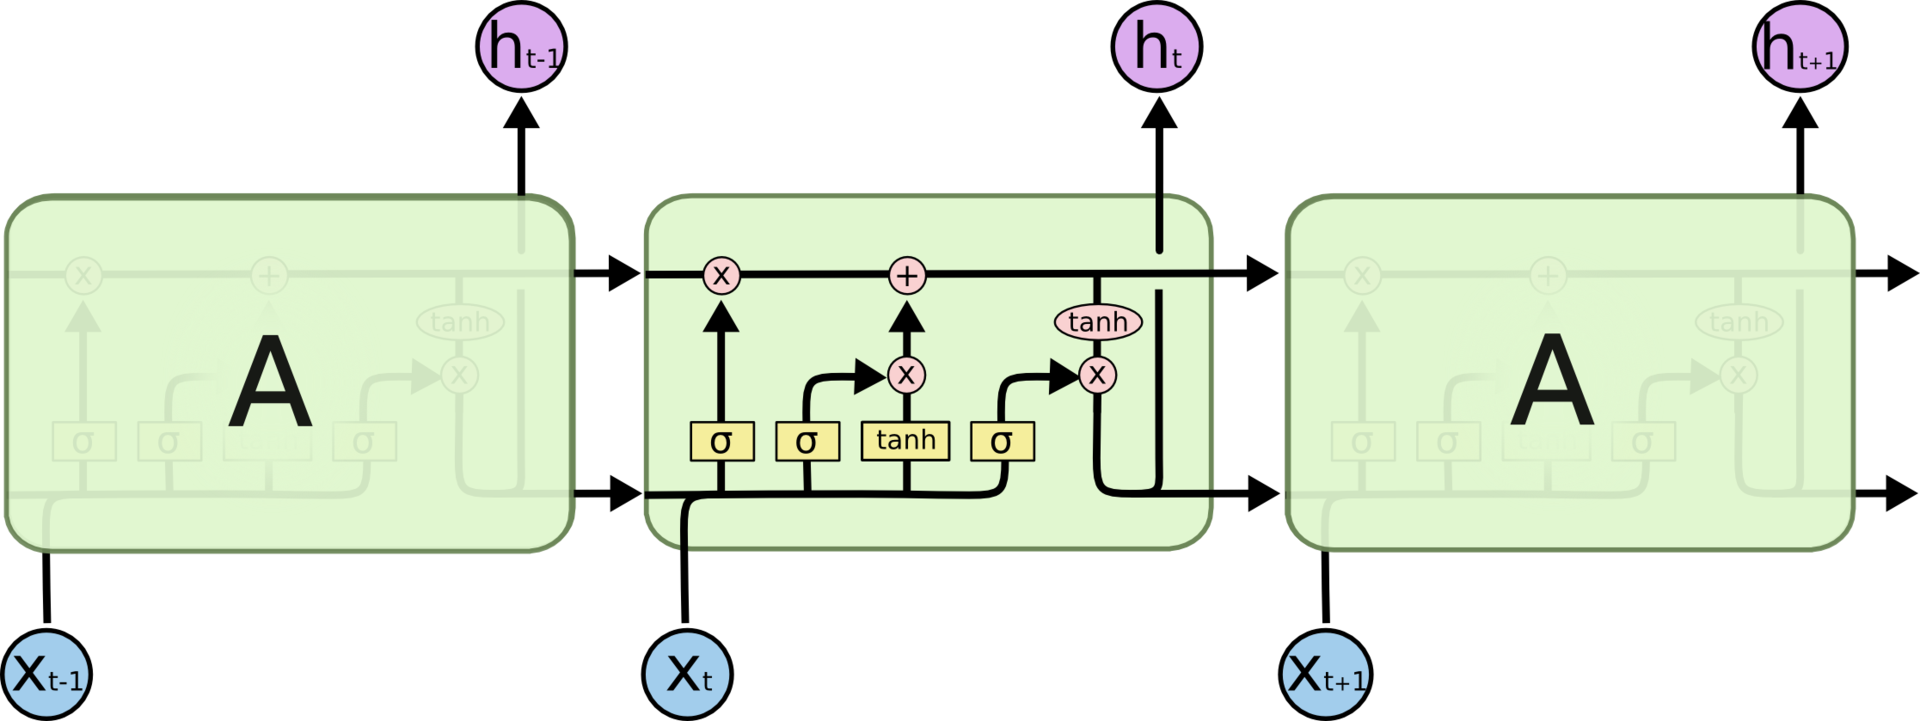
\includegraphics[width=0.95\linewidth]{img/lstm}
	\caption{Повторяющийся модуль в LSTM сети}
	\label{fig:lstm}
\end{figure}

В приведенных выше преобразованиях ячейка памяти $ c_t $ хранит «долгосрочную» память в векторной форме. Другими словами, информация накапливается и кодируется до тех пор, пока временной интервал $ t $ не будет сохранен в $ c_t $ и будет передаваться только через один и тот же уровень на разных временных шагах.
Учитывая входы $ c_t $ и $ h_t $, вход и “забывающий” элемент $ f_t $ помогут ячейке памяти решить, как перезаписать или сохранить информацию в памяти. Выходной шлюз далее позволяет блоку LSTM решить, как получить информацию о памяти для генерации текущего состояния $ h_t $, которое передается как на следующий уровень текущего временного шага, так и на следующий шаг времени текущего уровня. Такие решения принимаются с использованием параметров скрытого слоя $ W $ и $ b $ с разными индексами: эти параметры будут выведены на этапе обучения сети.

\subsection{Архитектура Модели}
Основная структура нашей модели такова:
учитывая изображение, мы извлекаем вектор признаков изображения (до слоя SoftMax) в PlaNet. Этот вектор подается в блок LSTM. Выходной вектор LSTM затем подаётся в слой SoftMax, который
выполняет классификацию в ячейки S2. Мы подаём альбом в модель в хронологическом порядке. В генерации признаков мы переиспользуем параметры модели для одиночного изображения. Во время обучения мы сохраняем их фиксированными и только обучать параметры LSTM и слой SoftMax.


Проблема с этой простой моделью LSTM заключается в том, что многие
альбомы содержат вначале несколько изображений, которые
не содержат полезной визуальной информации. Благодаря своей однонаправленности эта модель не может исправить неверные прогнозы, что
происходят в начале последовательности после наблюдения
фото с уверенным местоположением. По этой причине мы сейчас
оценить модель, в которой LSTM использует множество фотографий
от альбома, прежде чем сделать свое первое предсказание.
Смещение метки. Идея этой модели состоит в том, чтобы сдвинуть 
поиск поисков, что вывод отложен на несколько временных шагов. Основная мотивация этой идеи состоит в том, что
модель может накапливать информацию из нескольких изображений в
последовательность перед предсказаниями. Тем не менее, мы
обнаружили, что использование смещений не улучшает локализацию
(Таблица 4, LSTM off1, LSTM off2). Предположим, что
из-за ввода входного изображения на выходные метки
становится более сложным, затрудняя прогнозирование
для всех фотографий, улучшая прогнозы только для конечности
количество фотографий. Более того, этот подход не
решить проблему повсеместно: например, если мы компенсируем
метка на 2 шага, но первое изображение
Фертильность возникает только после 3 шагов, прогноз для первого
изображение, вероятно, все еще будет неправильным. Чтобы исправить это, теперь мы сидером, которые определяют их прогнозы на всех изображениях
в последовательности, а не только предыдущие. Повторяющиеся последовательности. Сначала мы оцениваем модель, которая
обученный по последовательностям
включая два экземпляра одной и той же последовательности. для эта модель, мы принимаем только прогнозы для изображений из вторая половина последовательности (т. е. повторяющаяся часть).

При времени вывода, передавая последовательность в модель
в первый раз можно рассматривать как стадию кодирования, где
LSTM создает внутреннее состояние на основе изображений.
Второй проход представляет собой этап декодирования, где на каждом изображении,
LSTM делает прогноз на основе его состояния,
аренда изображение. Результаты показывают, что этот подход превосходит
однопроходные LSTM, достигающие 7,8\%
относительное улучшение на уровне улицы, ценой двоякого
увеличение времени вывода. Однако,
В результате мы обнаружили проблему с этим подходом:
если в начале
последовательности, они, как правило, привязаны к последнему
катиона в последовательности, поскольку модель учится полагаться на
его предыдущее предсказание. Поэтому прогнозы с конца
последовательности переносятся в начало.
Двунаправленный LSTM. Известная нейронная сеть ar-
архитектуры, которая обусловливает прогнозы в целом
последовательности являются двунаправленными LSTM (BLSTM). Эта модель можно рассматривать как конкатенацию двух моделей LSTM, где первая выполняет передний проход, а вторая выполняет обратный проход по последовательности. Двунаправленные LSTM не могут быть обучены с помощью обратного распространения во времени с усечением и, следовательно, для LSTM до полной длины последовательности. Чтобы уменьшить
вычислительную стоимость обучения, нам пришлось ограничить продолжительность
последовательности до 25 изображений. Это приводит к снижению общей
точности, поскольку более длинные альбомы обычно дают
большую точность чем короткие. Поскольку наши эксперименты по этим данным
не сопоставимы с предыдущими, мы также
оценили повторяющуюся модель LSTM на усеченных последовательностях
до 25 изображений. Как показывают результаты BLSTM явно превосходят повторные LSTM
(Относительное улучшение на уровне улицы на 16,6\%). Однако,
потому что они не подходят для длинных последовательностей, повторяющиеся модель может быть предпочтительнее на практике.


\section{Разработка метода геолокации по серии изображений используя выбранные/разработанные выше алгоритмы/методы}

\section{Выводы}

Необходимо перечислить, какие теоретические результаты были получены с 
указанием степени новизны. Например: <<Была разработана такая-то модель. Она 
представляет собой адаптированную версию модели $X$, в которой уравнение $Z$ 
заменено на уравнение $Z'$>>. Еще пример: <<Была предложена такая-то 
архитектура, она отличается от типовой в том-то и том-то. Это позволяет 
избежать таких-то проблем.>>. При этом не следует заниматься <<высасыванием из 
пальца>>: <<Поставленная задача является типовой; для ее решения применены 
стандартные средства (перечислить, какие).>>.
